\documentclass[9pt]{beamer}

\usepackage[T1]{fontenc}
\usepackage{color}
\usepackage{graphicx}
\usepackage{natbib}
\usepackage{bibentry}
\usepackage{tikz}
\usepackage{xmpmulti}
\usepackage{animate}
\usepackage{tcolorbox}

\usetheme{Boadilla}

\usefonttheme{professionalfonts}

\graphicspath{C:/Users/galm/Documents/papers/sustainability/plots}

\title[Apsis Tools]{Topic Modelling}
\subtitle{}
\author{Max Callaghan}
\institute[MCC]{
	%
\includegraphics[height=1cm,width=2cm]{/home/max/Pictures/MCC_Logo_RZ_rgb.jpg}
	
\includegraphics[height=1cm,width=2cm]{images/MCC_Logo_RZ_rgb.jpg}
}

\bibliographystyle{apalike}

\begin{document}
	
	\begin{frame}
	\titlepage
\end{frame}


\begin{frame}{Explanation}

With online archives of documents expanding, we have more information than we can humanly process, but we also have new opportunities for using this information in different ways, or doing ``distant reading'' \citep{Moretti2013}.

\bigskip

\bigskip

Topic modelling describes ``a suite of algorithms that aim to discover and annotate large archives of documents with thematic information'' \citep{Blei2012}

\bigskip

\bigskip

This annotated corpus of documents allows us ``organise and summarise'' electronic text collections, so that we can ask questions about how themes are connected and have changed over time \citep{Blei2012}
\end{frame}

\begin{frame}{Words, Words, Words}

\begin{columns}
	\begin{column}{0.3\linewidth}
		\begin{itemize}
			\item<1->For topic modelling, a collection of documents is a matrix of word occurrences in documents
			\item<1->(The bag of words assumption)
		\end{itemize}
		
	\end{column}
	\begin{column}{0.7\linewidth}
		\only<1->{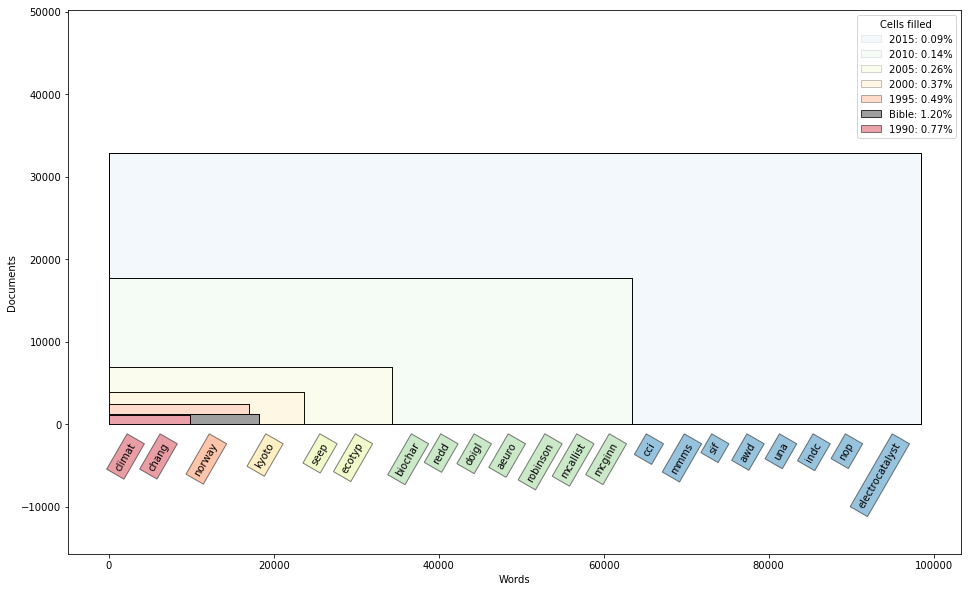
\includegraphics[width=\linewidth]{images/volume_variety_bible.png}}
	\end{column}
\end{columns}
	
\end{frame}


\begin{frame}{Non-negative Matrix Factorisation (NMF)}

\citep{Lee1999}

\begin{figure}
	
	\[V_{i\mu} \]
	
	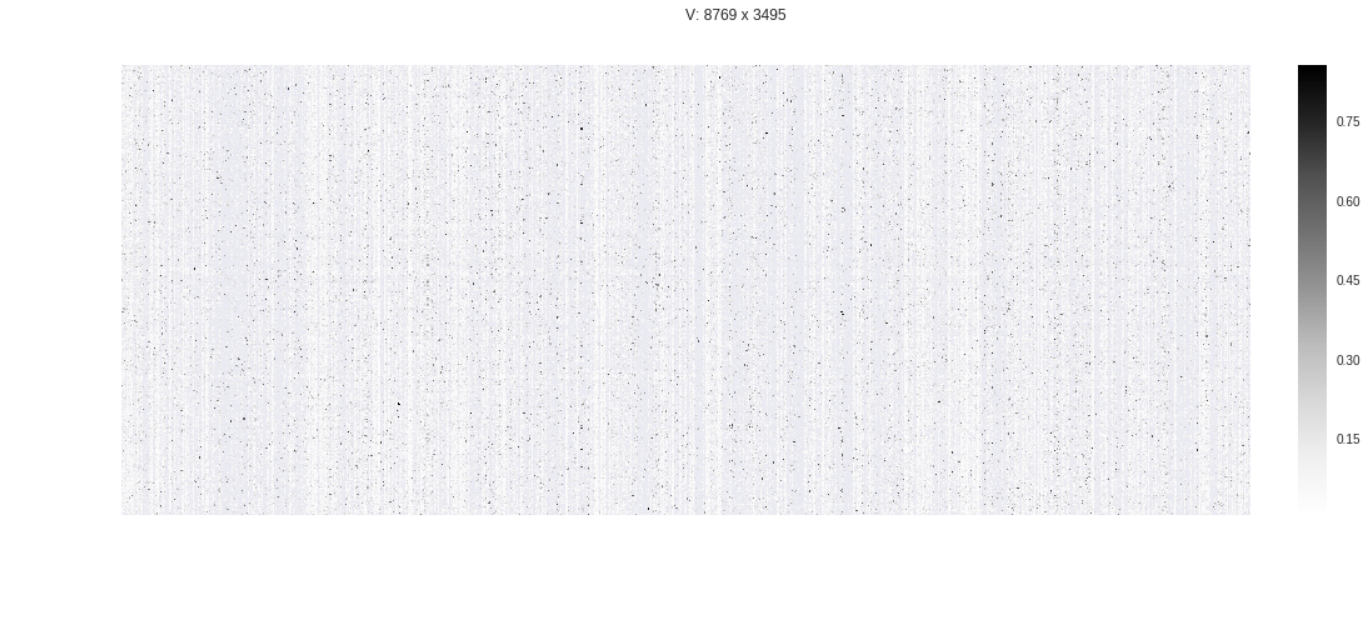
\includegraphics[width=\linewidth]{images/VWH_blank.png}
	
	\caption{A Document term matrix of 3495 documents on climate change from the year 2000}
	
\end{figure}

\end{frame}


\begin{frame}{Non-negative Matrix Factorisation (NMF)}

\citep{Lee1999}

\begin{figure}

\[V_{i\mu} \approx (WH)_{i\mu} = \sum_{a=1}^{r}W_{ia}H_{a\mu} \]

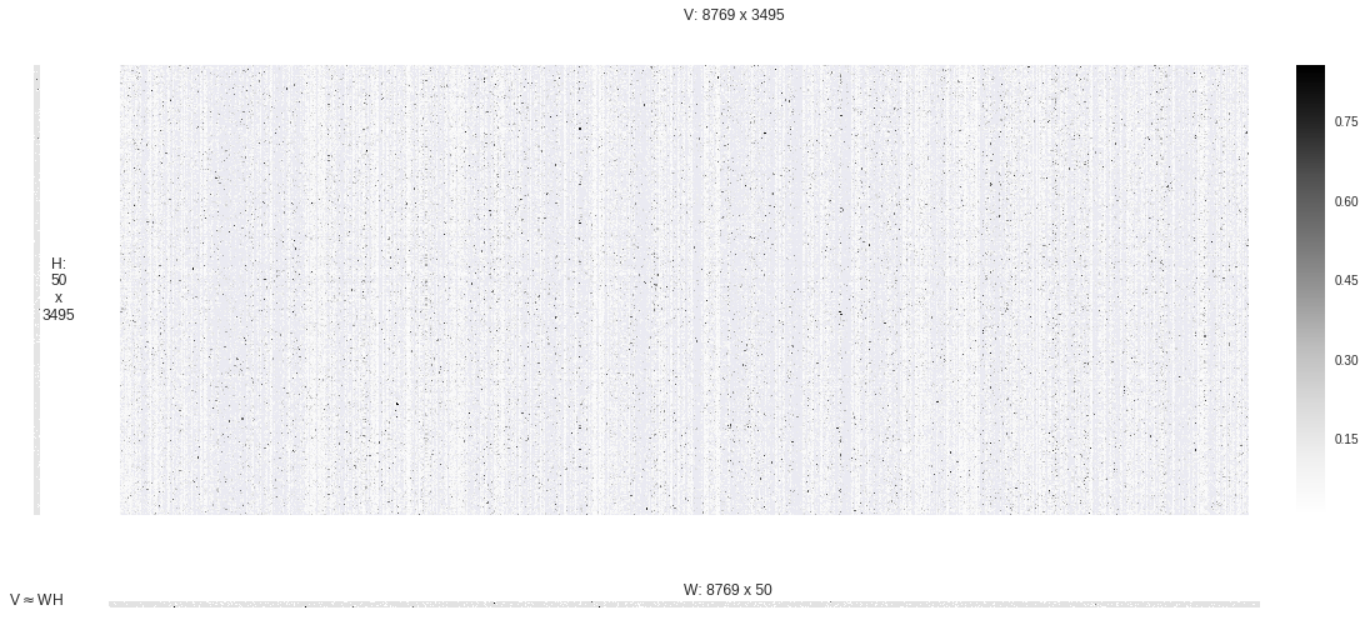
\includegraphics[width=\linewidth]{images/VWH.png}

	\caption{A topic model of 3495 documents on climate change from the year 2000}

\end{figure}


\end{frame}


\begin{frame}{Latent Dirichlet Allocation (LDA)}

\begin{columns}
	\begin{column}{0.45\linewidth}
		\only<1->{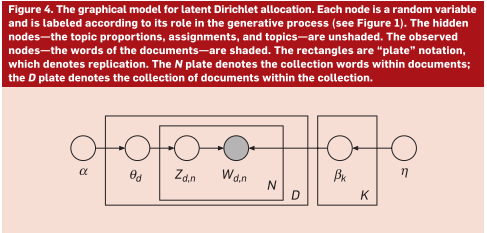
\includegraphics[width=\linewidth]{images/blei2012-4.png}}
	\end{column}

	\begin{column}{0.55\linewidth}	
	\begin{itemize}
		\item<1->LDA similarly describes documents as distributions of topics, which are distributions of words
		\item<1->The assumptions about probability are slightly different, but the intuition is the same
	\end{itemize}
	
	\end{column}
\end{columns}

\centering

\only<1->{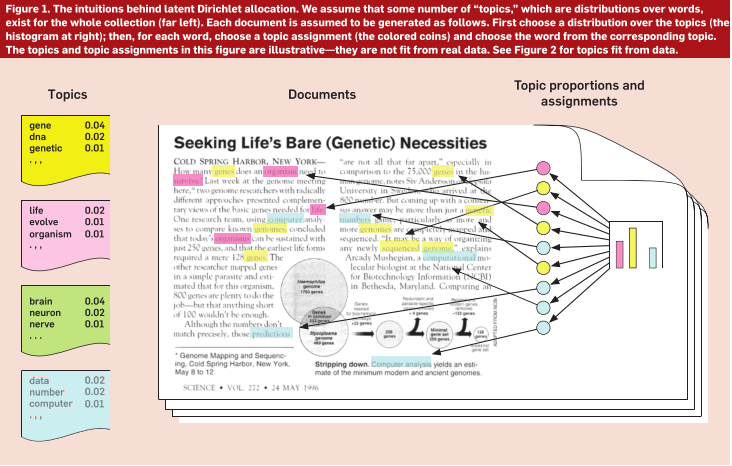
\includegraphics[width=0.7\linewidth]{images/blei2012-1.png}}

\end{frame}

\begin{frame}{APSIS applications - NETs}

\nobibliography*

\begin{columns}
	\begin{column}{0.65\linewidth}
		\begin{figure}
			\only<1->{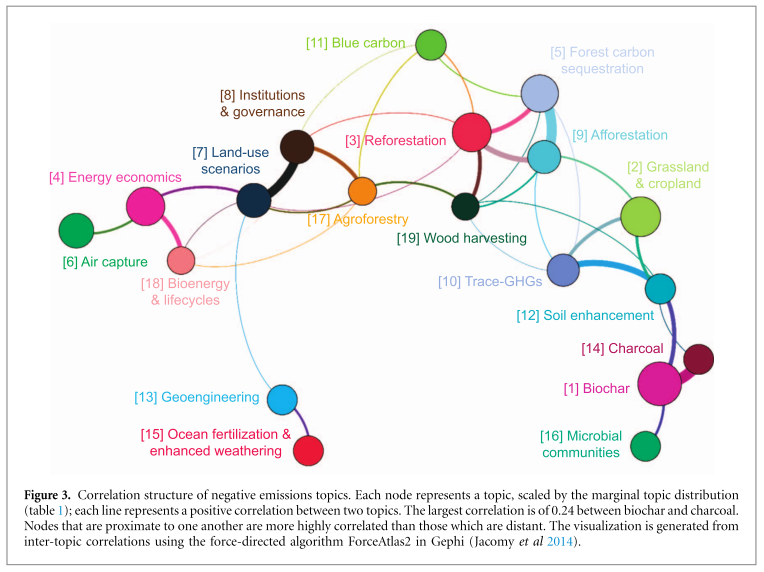
\includegraphics[width=\linewidth]{images/minx2017n-3.png}}
			\caption{\bibentry{Minx2017c}}
		\end{figure}
		
	\end{column}
	
	\begin{column}{0.35\linewidth}	
		\begin{itemize}
			\item<1->What topics exist on negative emissions, how are they connected? 
			%\item<1->
		\end{itemize}
		
	\end{column}
\end{columns}

\end{frame}

\begin{frame}{APSIS applications - Cities}

\nobibliography*

\begin{columns}
	\begin{column}{0.65\linewidth}
		\begin{figure}
			\only<1->{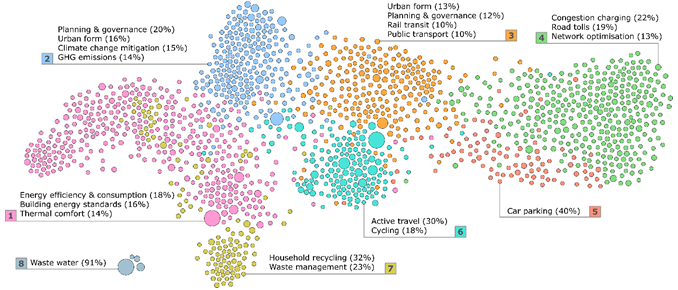
\includegraphics[width=\linewidth]{images/lamb2017-4.png}}
			\caption{\bibentry{Lamb2017} (Submitted)}
		\end{figure}
		
	\end{column}
	
	\begin{column}{0.35\linewidth}	
		\begin{itemize}
			\item<1->Topics can be used to characterize bibliographic networks
			%\item<1->
		\end{itemize}
		
	\end{column}
\end{columns}

\end{frame}

\begin{frame}{APSIS applications - Cities}


		\begin{figure}
			\only<1->{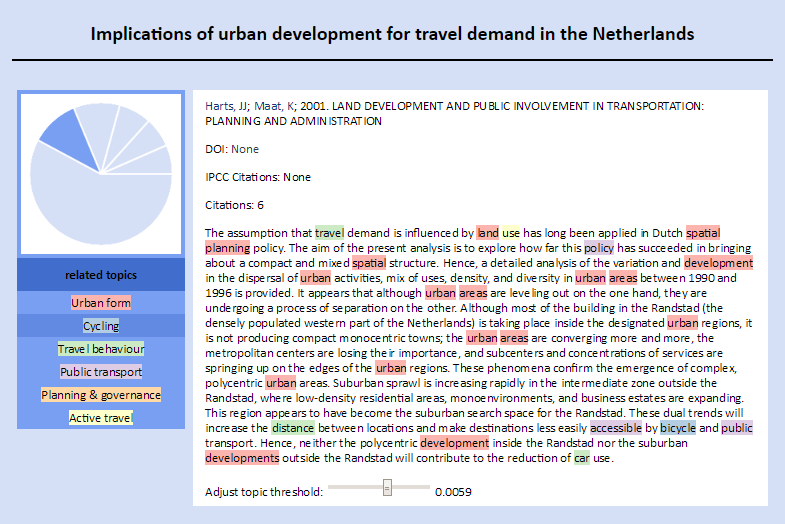
\includegraphics[width=0.8\linewidth]{images/lamb2017-paper.png}}
			\caption{Annotated document using data from \citet{Lamb2017} }
		\end{figure}


\end{frame}

\begin{frame}{APSIS applications - Cities}


\begin{figure}
	\only<1->{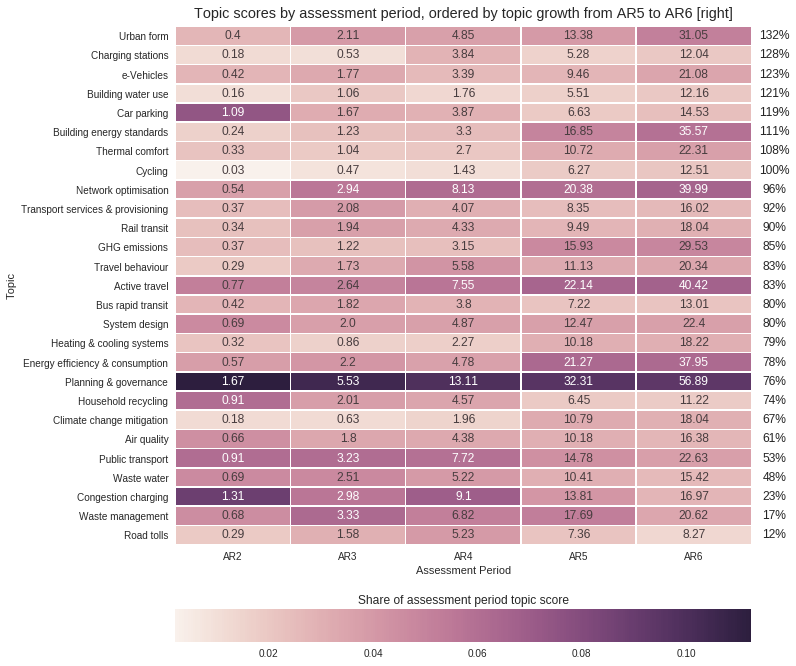
\includegraphics[width=0.7\linewidth]{images/topic_ap_normalised_growth_shares.png}}
	\caption{Topic Growth over time \citep{Lamb2017} }
\end{figure}


\end{frame}

\begin{frame}{Extensions}

\begin{columns}
	\begin{column}{0.5\linewidth}
		\begin{tcolorbox}[colback=green!5,colframe=green!40!black]
			Incorporating additional information
		\end{tcolorbox}
		\begin{itemize}
			\item Place mentions / IPCC references
			\item Structural topic models \citep{Roberts2014a}
		\end{itemize}	
	\end{column}
	
	\begin{column}{0.5\linewidth}	
		\begin{tcolorbox}[colback=green!5,colframe=green!40!black]
			Better modelling topic dynamics
		\end{tcolorbox}
		\begin{itemize}
			\item Emergence / Evolution of topics
			\item Dynamic landscape of sustainability \citep{Minx2017} 
			%\item<1->
		\end{itemize}
		
	\end{column}
\end{columns}

\end{frame}

\begin{frame}{Dynamic Topic Models}

%\begin{tcolorbox}[colback=green!5,colframe=green!40!black]
%	Better modelling topic dynamics
%\end{tcolorbox}

\begin{columns}
	\begin{column}{0.5\linewidth}
		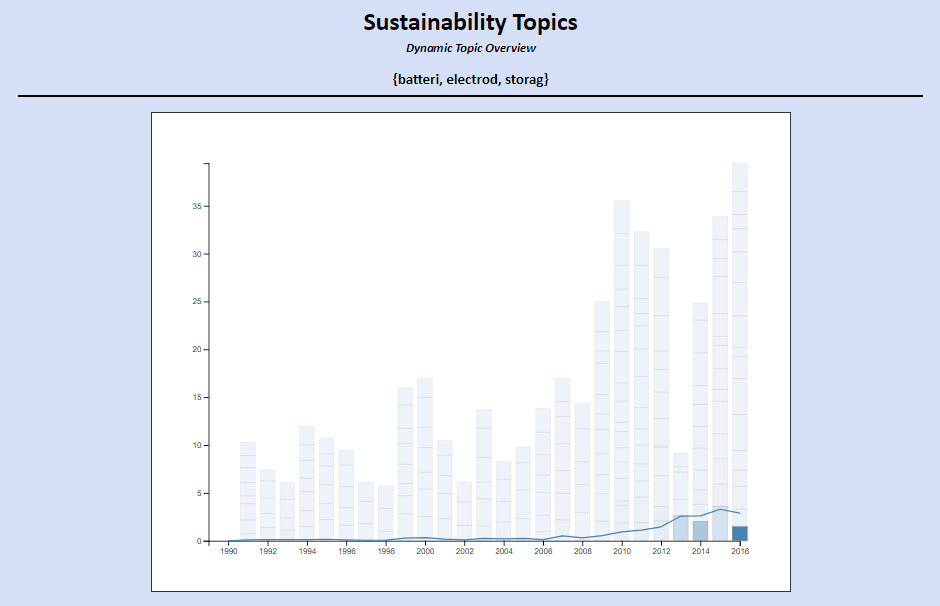
\includegraphics[width=\linewidth]{images/sus_batteries.png}
	\end{column}
	
	\begin{column}{0.5\linewidth}	
		In \citep{Minx2017} we apply \citet{Greene2016}' Dynamic Topic Model
	\end{column}
\end{columns}

\bigskip

	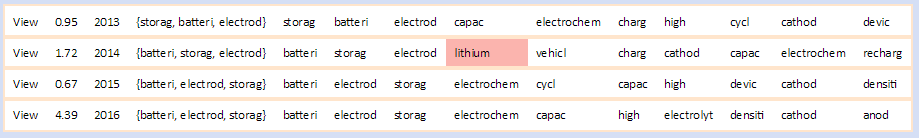
\includegraphics[width=\linewidth]{images/sus_batteries_words.png}	

\end{frame}

\begin{frame}[t]{Dynamic Topic Models}

\only<1->{\includegraphics[]{C:/Users/galm/Documents/papers/sustainability/plots/VWH_1991}}
\only<2->{\includegraphics[]{C:/Users/galm/Documents/papers/sustainability/plots/VWH_1992}}

\only<3->{\includegraphics[]{C:/Users/galm/Documents/papers/sustainability/plots/VWH_1993}}

\end{frame}

\begin{frame}[t]{Dynamic Topic Models}

\includegraphics[width=\linewidth]{C:/Users/galm/Documents/papers/sustainability/plots/conceptual_windows_only}

\end{frame}

\begin{frame}[t]{Dynamic Topic Models}

\includegraphics[width=\linewidth]{C:/Users/galm/Documents/papers/sustainability/plots/conceptual_annotated_1}

\end{frame}

\begin{frame}[t]{Dynamic Topic Models}

\includegraphics[width=\linewidth]{C:/Users/galm/Documents/papers/sustainability/plots/conceptual_annotated_2}

\end{frame}

\begin{frame}{Other Text Analysis}

\begin{columns}
	\begin{column}{0.5\linewidth}
		\begin{center}
			\fbox{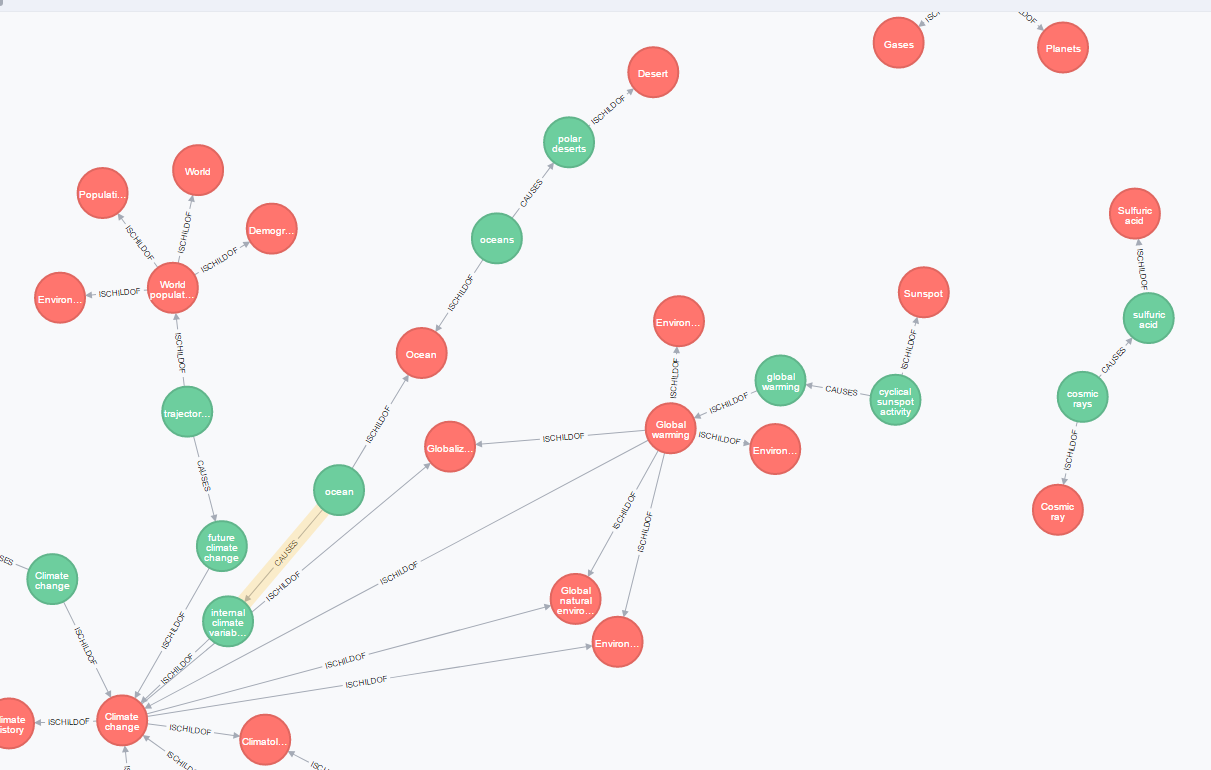
\includegraphics[width=\linewidth]{images/extract_raw.png}}
		\end{center}
	\end{column}
	\begin{column}{0.5\linewidth}
		\begin{center}
			\begin{itemize}
				\item Causaly collect causal statements from literature
				\item They aim to quantify and aggregate the strength of claims
				
			\end{itemize}
			\medskip
			\textbf{Applications?}
			\begin{itemize}
				\item Do we get more consolidated knowledge about causal relationships over time (in some WGs over others)?
				\item What can we learn about co-benefits and side-effects of different negative emission technologies?
				
				
			\end{itemize}
		\end{center}
	\end{column}
\end{columns}

\end{frame}



\begin{frame}{Bibliography}
\small
%\bibliography{/home/max/Documents/library/bibliography}
\bibliography{C:/Users/galm/Documents/library/library}
\end{frame}


\end{document}